\chapter{Control Unit}
\label{chap:cu}

The DLX's control unit is mainly based on the hardwired approach, although some operations are handled by in-stage FSMs. The former approach has been chosen
because most of the control signals of an operation never changes during its execution. For example, for an \verb|add| instruction the value of \verb|rp1_out_sel|
is always \verb|00| and will never change, no matter what happens in the pipeline. Because of this, reading the values from a control register and writing them directly in the
component is the fastest and cheapest way to control the datapath. However, not all the signals can be known a-priori, or they need to change over time to handle complex operations:
the former case is represented by the forwarding signals for example, while the latter from the multiplication. Due to this we had to resort to in-stage FSM able to correctly manage
these situations.

The control unit is by far the most complex component in the DLX, therefore to ease the explanation the rest of the chapter is divided in sections, each of which explains what happens
in the related stage. 

\section{IF stage}
\label{sec:cu_IF_stage}

The PC register in the datapath is used to access the {\it instruction ROM}, or IROM, where all the instructions to be executed are stored. The IROM's output is then sent to both the
control unit, to analyze the instruction's {\it opcode} and {\it func} fields, and to the IF/ID registers for decoding the rest of the fields in the ID stage.
The control units hosts two ROMs: one contains all the control words (also referred to as {\it CW}) related the I and J instructions, while the other one stores all the CW belonging
to the R instructions. The former is accessed using the opcode field, the latter using the func field. This distinction had to be done because all R instructions have the same opcode,
which is equal to \verb|0x00|.

\begin{figure}[!ht]
	\centering
	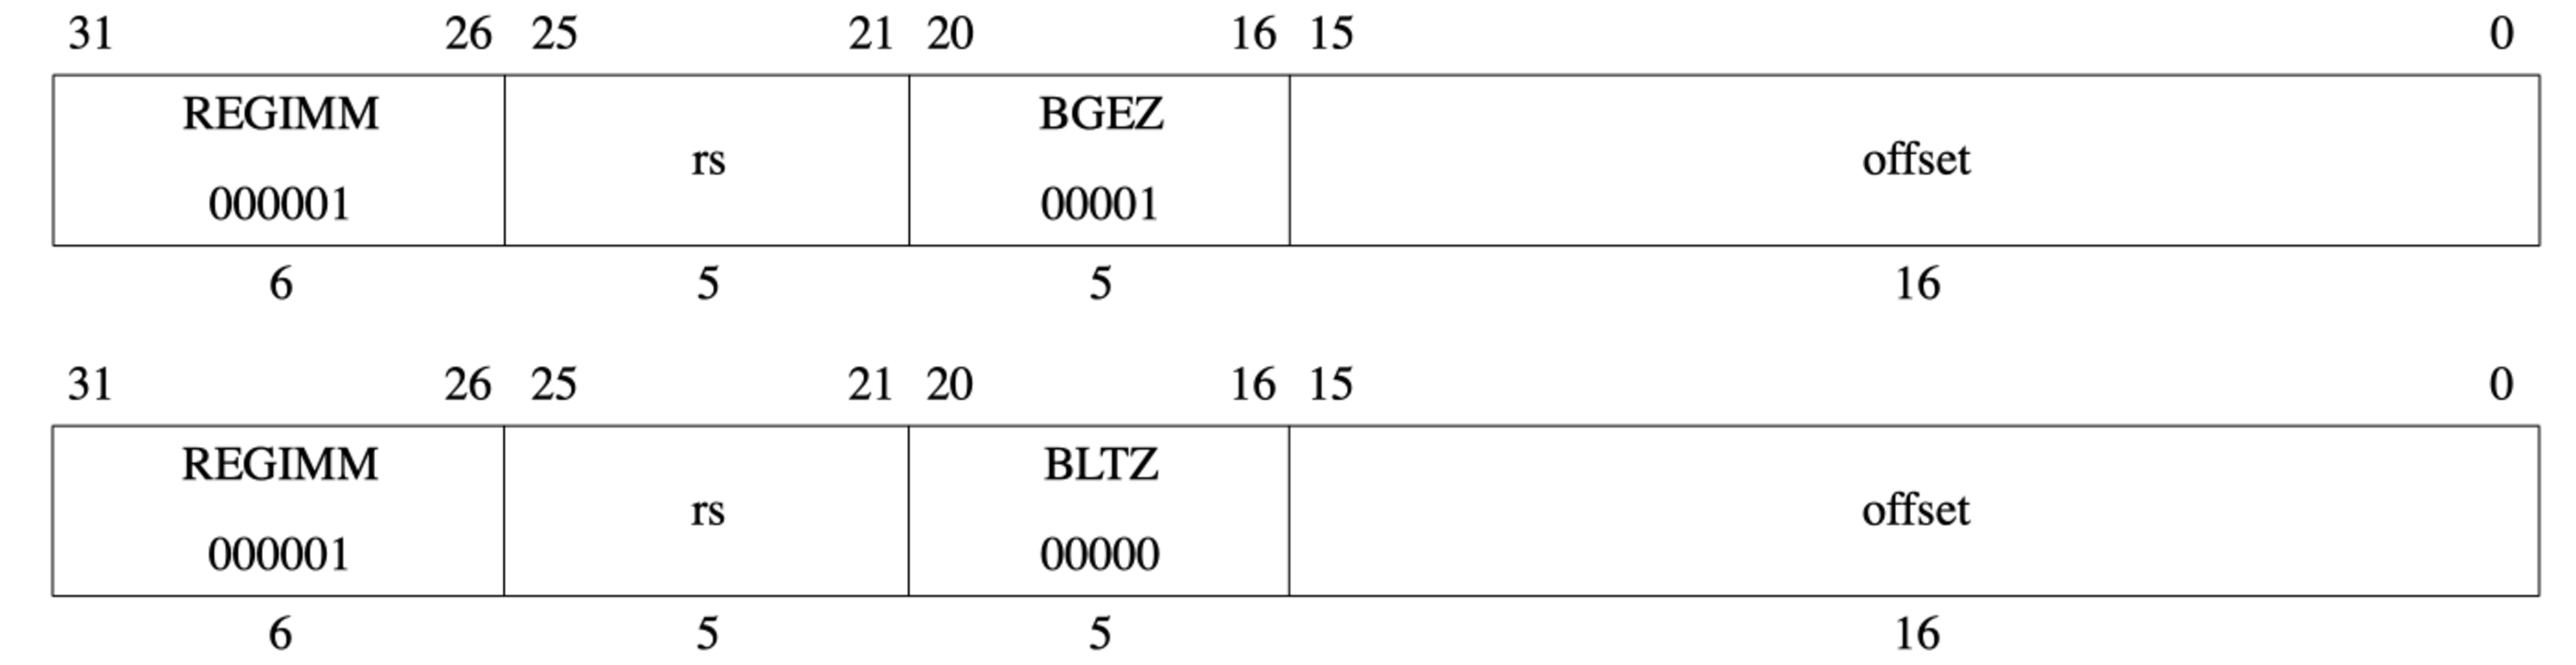
\includegraphics[width=\linewidth]{./chapters/figures/bltz_bgez.pdf}
    \caption{bltz and bgez instruction format. Taken from \cite{MIPS64_arch}}
    \label{fig:bltz_bgez}
\end{figure}

The control unit recognize this pattern and it chooses the right CW for each instruction. Nonetheless this is not the only particular case. As already shown in table \ref{tab:sup_instr},
\verb|bgez| and \verb|bltz| shares the same opcode. Their difference reside in the bits 20-16, which are set to \verb|00001| for the former, to \verb|00000| for the latter (figure \ref{fig:bltz_bgez}).
This information cannot be used to differentiate the branches directly in the CW's ROM, hence their final CW is generated dynamically.

This part of the control unit also decide from which source must come the next value of the PC register. Four cases have to be distinguished:

\begin{enumerate}
    \item The EXE stage have not executed a branch and the BTB predicts as not taken the current fetched instruction: in this case $PC + 4$ is chosen.
    \item The EXE stage have not executed a branch and the BTB predicts as taken the current fetched instruction: in this case $PC_{BTB}$ is chosen.
    \item The EXE has executed a \verb|jr| or a \verb|jalr|: the prediction of the BTB is discarded and $PC_{main\ adder}$ is chosen.
    \item the EXE has executed a branch or a jump different from \verb|jr| or \verb|jalr| and it was either unknown or mispredicted: the prediction of the BTB is discarded and $PC_{secondary\ adder}$ is chosen.
\end{enumerate}

\section{ID stage}

The bits used to drive the ID stage are all static, therefore they are directly read from the control unit's IF/ID register and are sent to the datapath. Here is it worth commenting
how this stage interacts with the EXE stage. When a multiplication is in progress in the EXE stage it is the EXE stage's FSM to drive the ID/EXE registers, therefore all the ID's signals
going to the ID/EXE registers are set in high impedance to avoid conflicts.

The ID stage is also in charge of detecting a \verb|mult| instruction, and when it does so it may need to stall the pipeline. Unfortunately, when the multiplication's operand are sent to the
ID/EXE stage, they are automatically extended on 64 bits by the registers themselves. This means that a \verb|mult| cannot enters the EXE stage if one of its source operands is still being processed
in the pipeline. Due to this limitation, when an hazard is detected for a multiplication, the control unit's ID stage in conjunction with the {\it stall unit} (explained in section \ref{sec:stall_unit})
stalls the IF and the ID stage, until all the data hazards have been resolved.

\section{EXE stage}
\label{sec:cu_exe_stage}

This is the biggest stage in the control unit's pipeline. It contains an FSM to handle the multiplication, which is the only instruction that requires more than a single clock cycle to execute.
Its state diagram is shown in figure \ref{fig:mul_fsm}.

\begin{figure}[!ht]
	\centering
	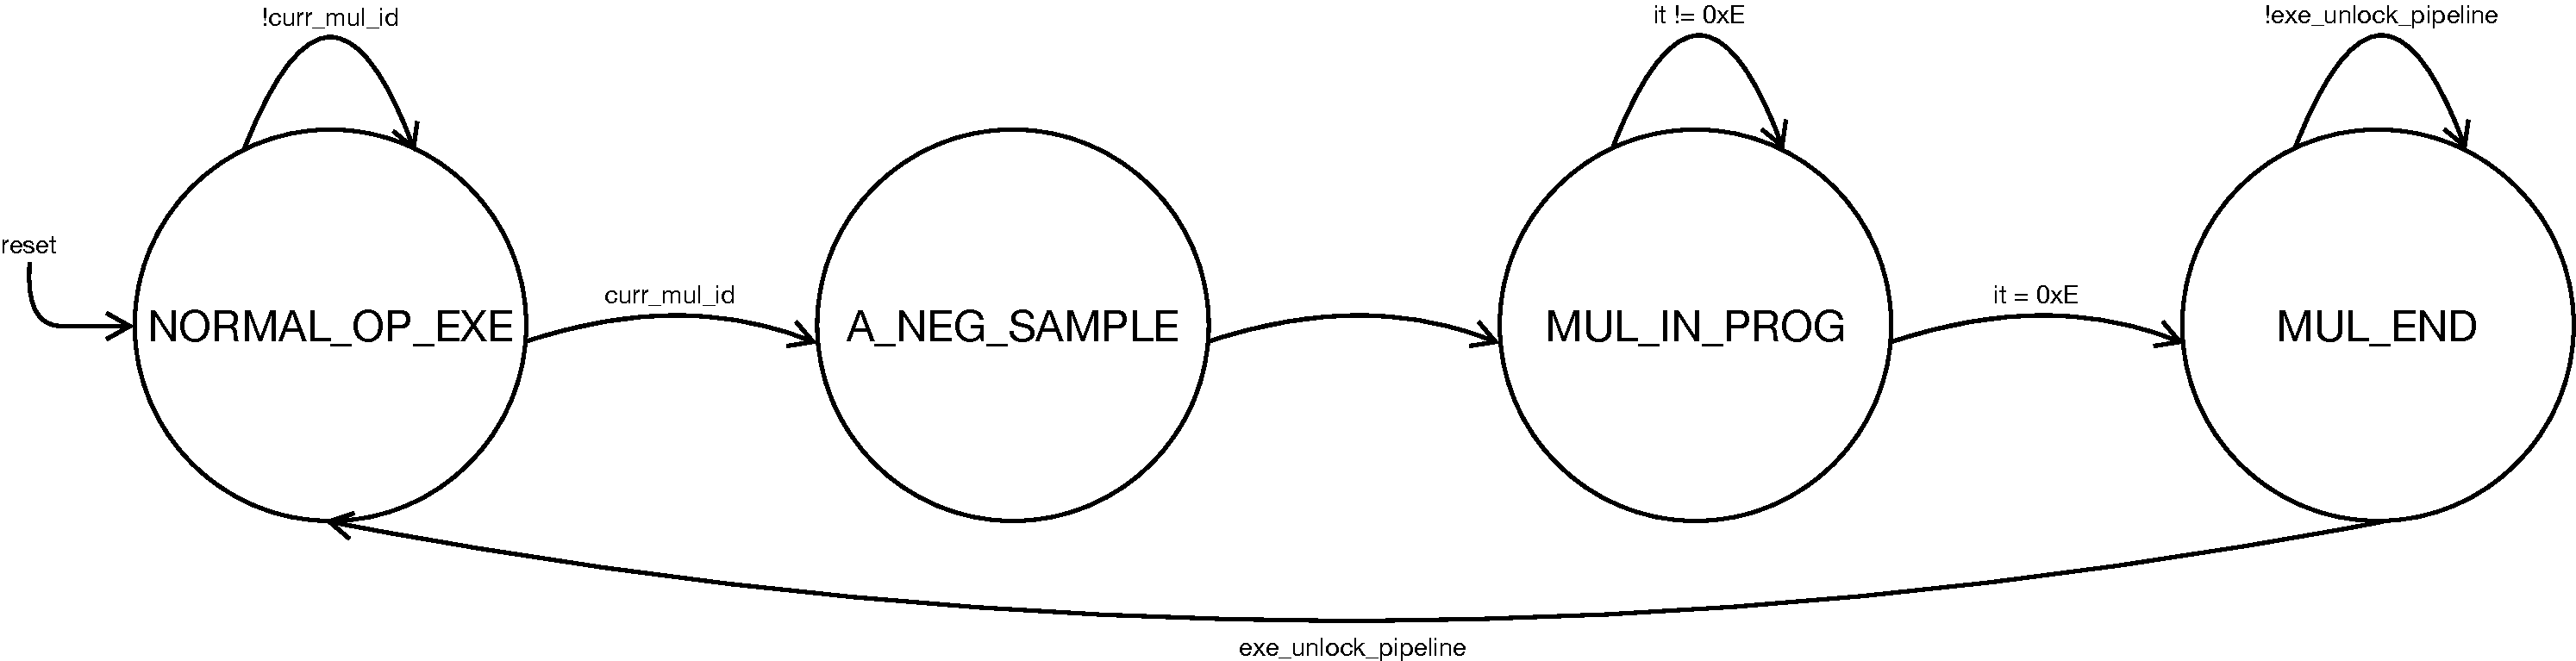
\includegraphics[width=\linewidth]{./chapters/figures/mul_fsm.pdf}
    \caption{EXE stage state diagram}
    \label{fig:mul_fsm}
\end{figure}

\subsection{NORMAL\_OP\_EXE}

This is the reset state and also the one where all the operations but \verb|mul| are executed. Here few checks are executed, therefore to ease the reader's understanding we have provided a flow diagram,
shown in figure \ref{fig:normal_op_flow_diagram}.

\begin{figure}[!ht]
	\centering
	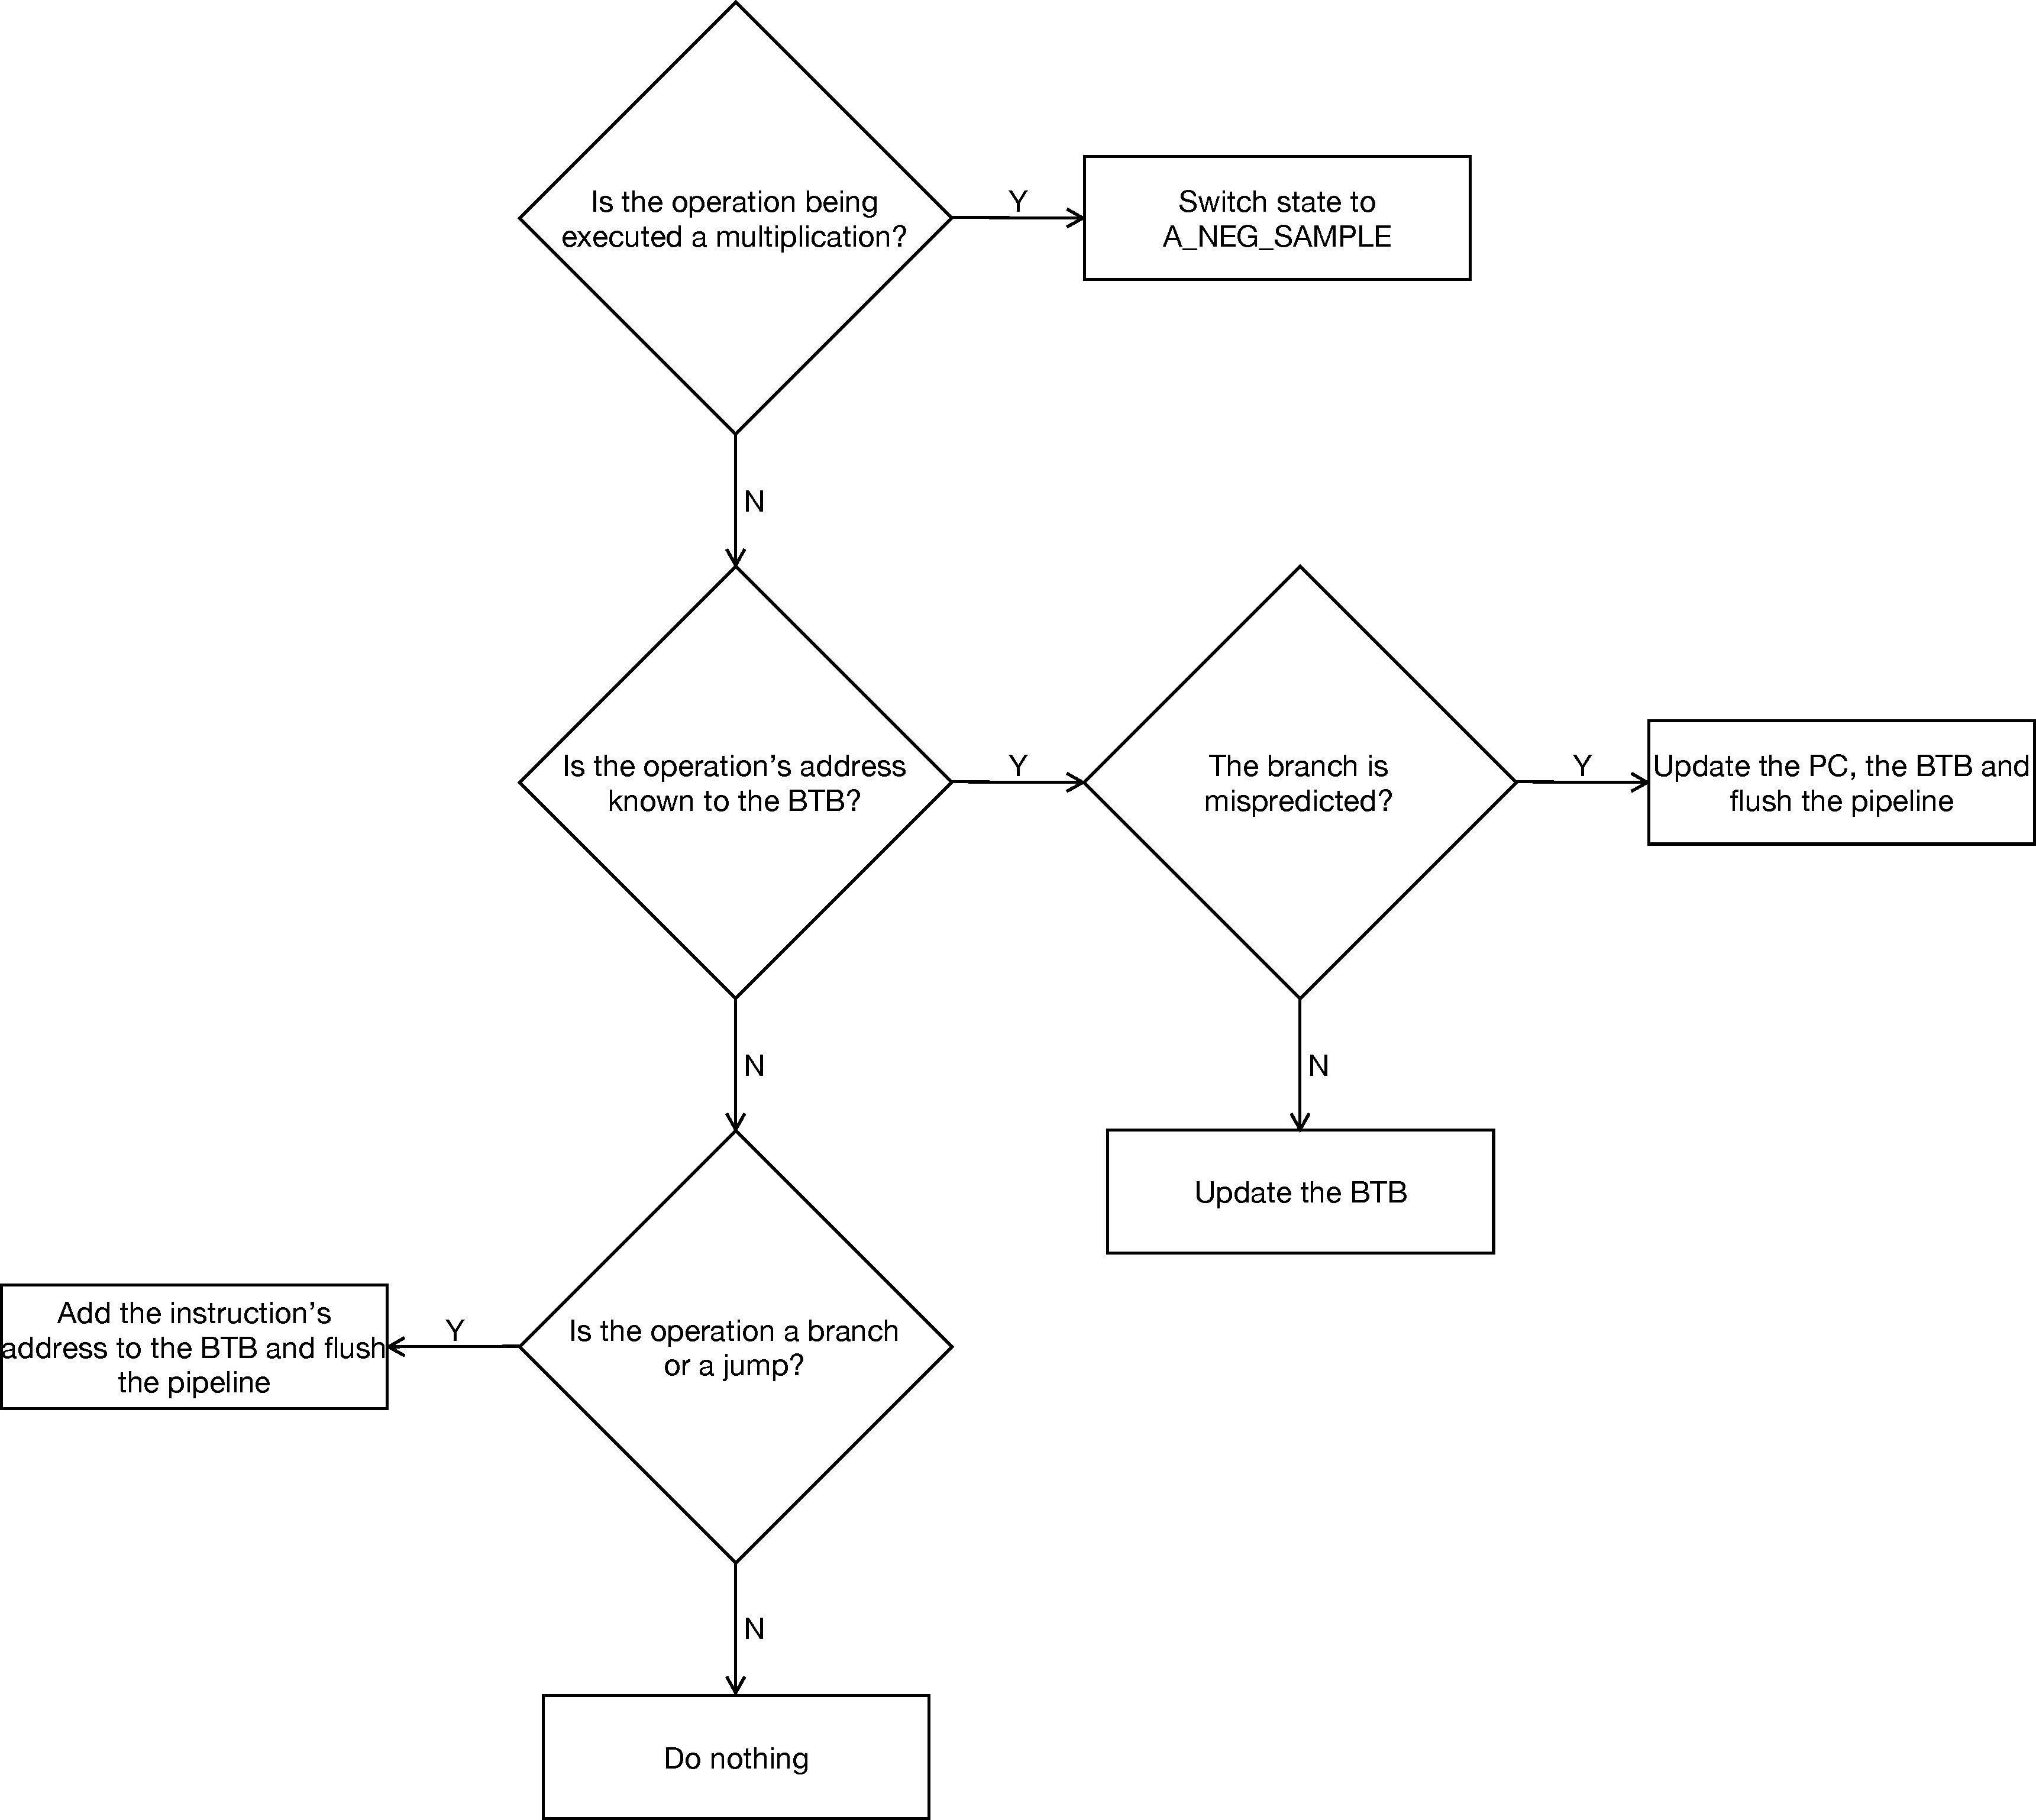
\includegraphics[width=\linewidth]{./chapters/figures/normal_op_diagram.pdf}
    \caption{NORMAL\_OP\_EXE flow diagram}
    \label{fig:normal_op_flow_diagram}
\end{figure}

The first check performed is whether the operation currently in the EXE stage is a multiplication or not. In the former case the EXE stage switch state as shown in figure \ref{fig:normal_op_flow_diagram} and stalls the pipeline,
while in the latter case the state remains unchanged. If the operation is not a multiplication, the other notable case is to check if the instruction is a branch or jump. To do so, it is controlled if the
BTB knew the instruction's address in the IF stage or not. If the address was known the only remaining check to be performed is whether the prediction was correct or not. In the first case the BTB prediction
is updated, otherwise besides the BTB's update the pipeline must be flushed and the PC changed.
If, instead, the address was not known, the FSM has to figure out if the instruction is a new branch or jump or not. In the latter case, besides writing as always the static control bits, nothing is done.
On the other hand, in the former case the address is added to the BTB, the pipeline is flushed and the PC is updated.

\subsection{A\_NEG\_SAMPLE}

This is the first state where the multiplication's execution starts. The EXE stage takes control over the ID/EXE registers, and uses the main adder to negate the value of the operand \verb|a| on 64 bits.
The next state of the FSM is automatically set to \verb|MUL_IN_PROG|.

\subsection{MUL\_IN\_PROG}

The FSM iterates over this state 15 times, using the multiplier's adder to calculate each time the partial result. As soon as the 15th iteration is executed, the next state is changed to \verb|MUL_END|.
In this state the EXE still controls the ID/EXE registers.

\subsection{MUL\_END}

This state is entered when the final result of the multiplication must be sampled by the EXE/MEM registers. After the result has been sampled, the EXE remains in this state (keeping therefore the pipeline locked)
until the multiplication result has reached the WB stage. When this happens, the next state of the FSM is set to \verb|NORMAL_OP_EXE| and the pipeline is unlocked.
Again, this shows a limitation of the \verb|mult|: its result cannot be forwarded to \verb|mflo| and \verb|mfhi| because it is on 64 bits and with our
forwarding logic only 32 bits can be forwarded. Hence, to maintain data flow correctness the multiplication's result must be sampled in the RF before the next instruction can enters the EXE stage.

\section{MEM stage}
\label{sec:cache_handling}

This stage, as all the previous ones, sends the static control bits to the datapath. When operations different from loads and stores pass through this stage, nothing more is done. Special attention must be
given to stores and, more importantly, to loads. In fact, the formers may generate cache evictions, while the latter ones may generate cache misses. Thanks to the design of the data cache and of the memory controller
cache eviction do not cause stalls, but cache misses do. Therefore, also in the MEM stage a FSM exists, of which the state diagram is shown in figure \ref{fig:mem_fsm}.

\begin{figure}[!ht]
	\centering
	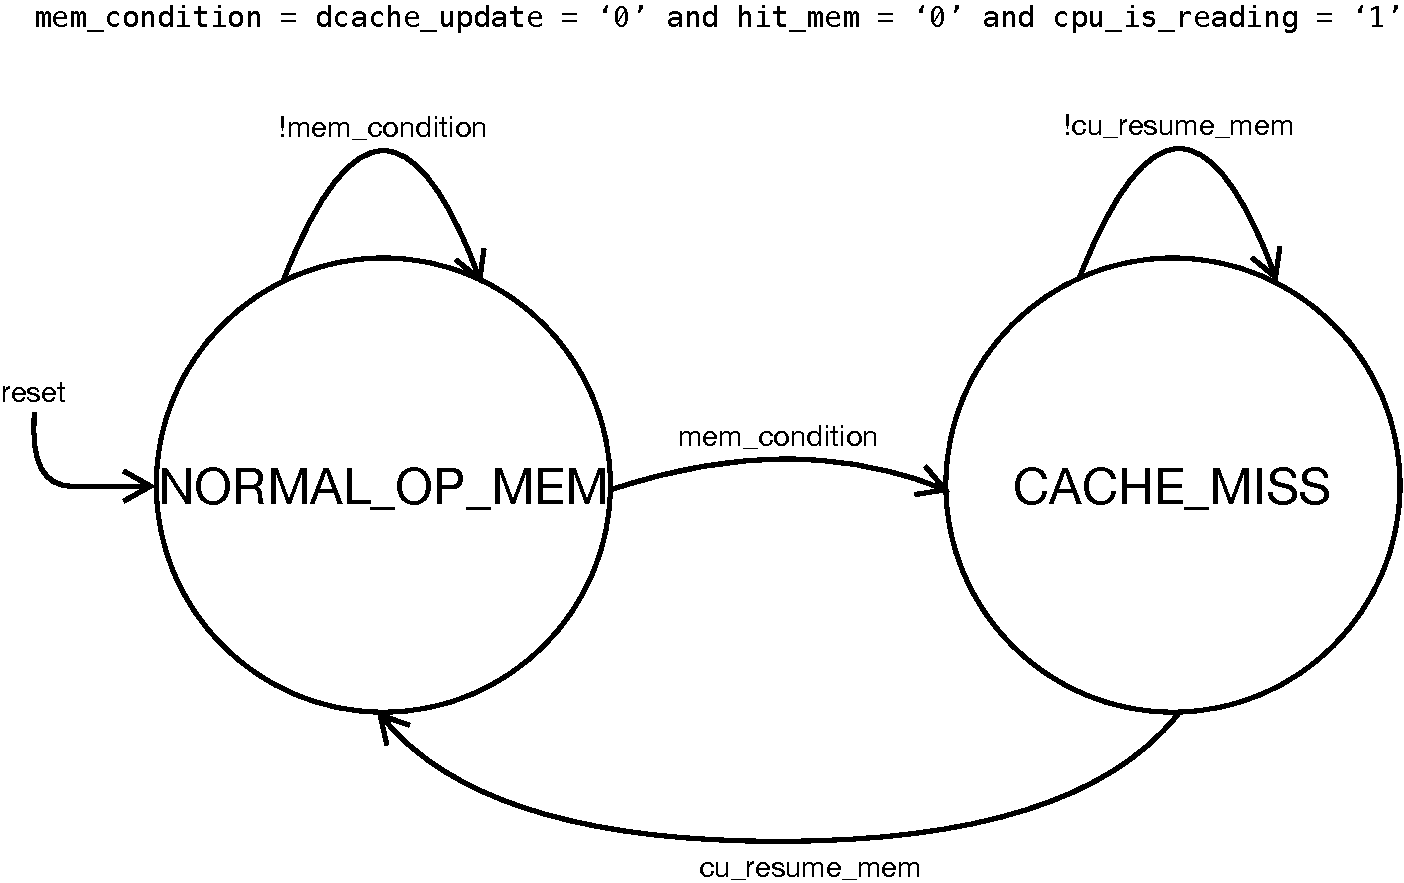
\includegraphics[width=0.5\linewidth]{./chapters/figures/mem_fsm.pdf}
    \caption{MEM stage state diagram}
    \label{fig:mem_fsm}
\end{figure}

\subsection{NORMAL\_OP\_MEM}

The FSM starts in this state and remains always here for all operations but loads. When a load is executed, the content indexed by the address may have been swapped out in cache, so the cache's \verb|hit| signal
would stay at 0. When this situation is detected, the MEM stage along with the stall unit stalls the entire processor and then sets the next state to \verb|CACHE_MISS|.

It is important to outline why \verb|mem_condition| in figure \ref{fig:mem_fsm} has that equation. Technically to detect the cache miss it would have been enough to look for \verb|dcache_update = 0 AND hit_mem = 0|, since
\verb|dcache_update| signals the processor's will to perform a read (by not updating anything in the memory) and \verb|hit_mem| signals if a hit or a miss have occurred. This is not sufficient however, because the cache is
accessed at every cycle using as address the output of the ALU, no matter if the instruction was actually a load or not. For this reason in the CW there is a field called \verb|cpu_is_reading|, which is set to 1 when the
processor wants to actually access the cache.

\subsection{CACHE\_MISS}
\label{subsec:cache_miss}

In this state the control unit hands over the control of the cache to the memory controller, which has recognized as well the cache miss in the previous cycle, by putting in high impedance \verb|dcache_update| and \verb|update_type_mem|.
The CU remains in this state as long as the memory controller does not raise the \verb|cu_resume| signal. When this happens, the pipeline is unlocked and the MEM stage FSM enters again the \verb|NORMAL_OP_MEM| state.

\subsubsection{Memory controller}

The memory controller resides outside the control unit. It acts as a communication layer for the cache and the RAM, moreover as said before is capable of resolving cache misses. It has its own FSM to perform its job,
shown in figure \ref{fig:memcontroller_fsm}.

\begin{figure}[!ht]
	\centering
	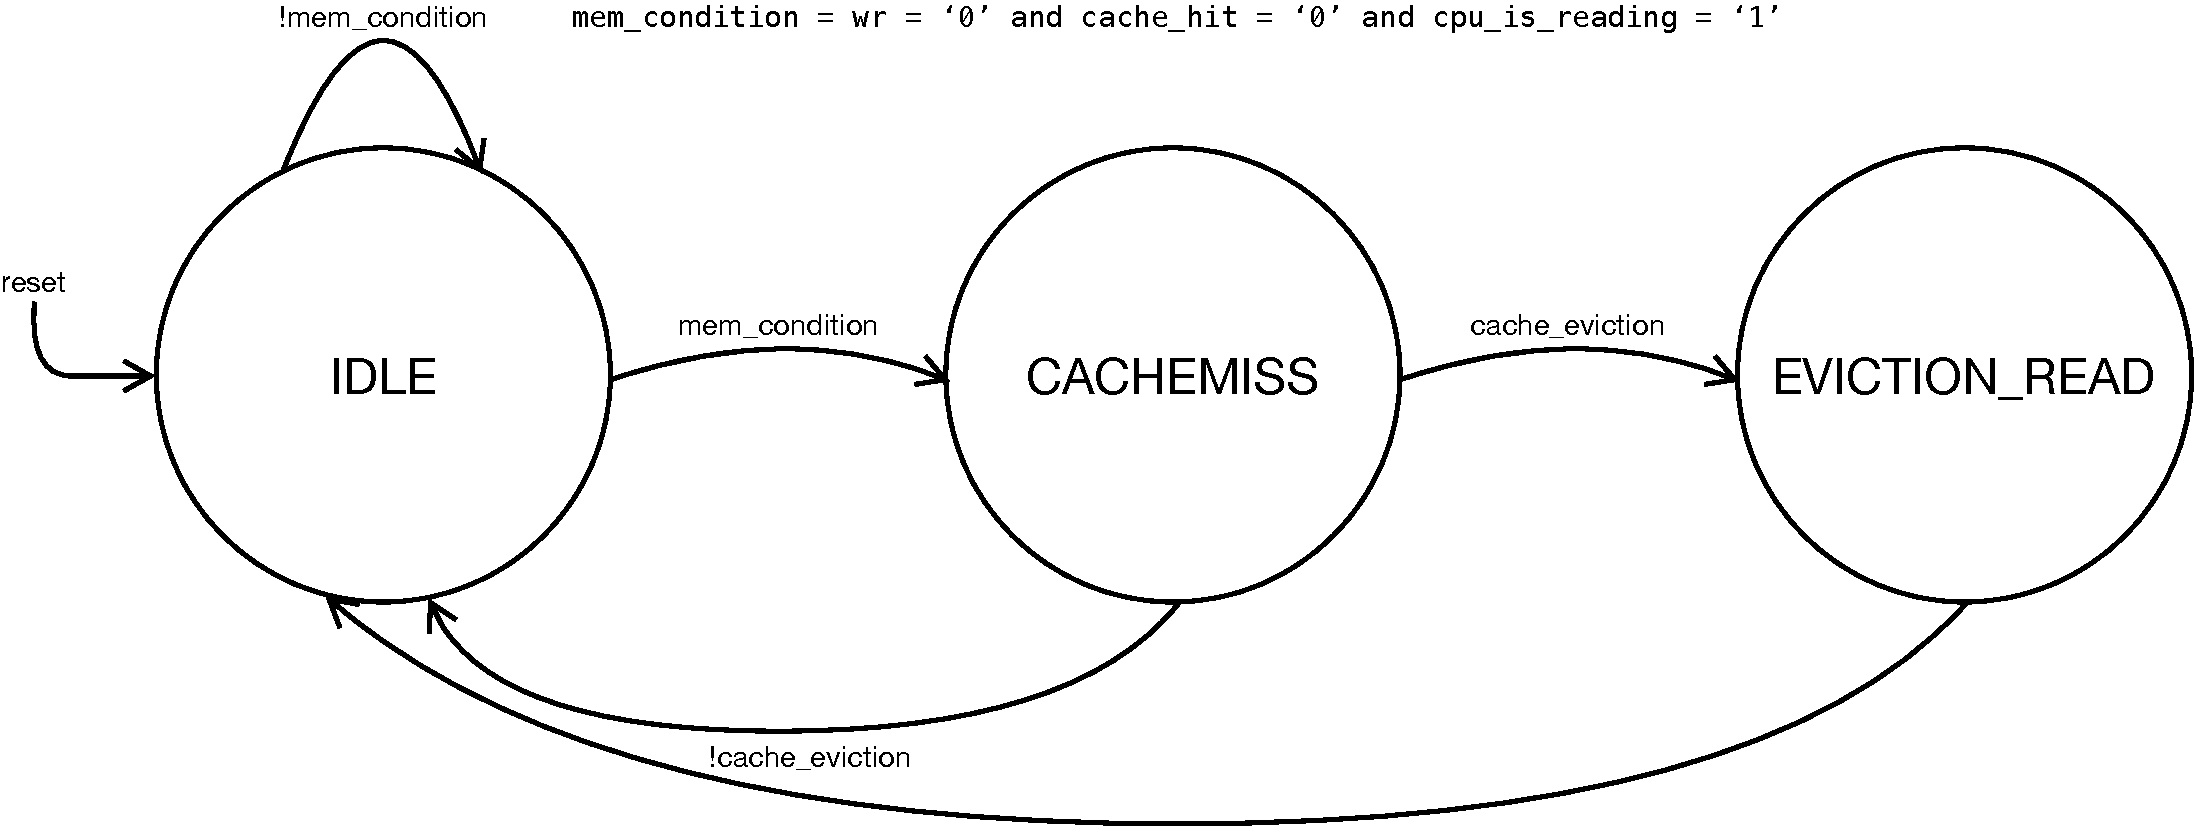
\includegraphics[width=0.8\linewidth]{./chapters/figures/memcontroller_fsm.pdf}
    \caption{Memory controller state diagram}
    \label{fig:memcontroller_fsm}
\end{figure}

\begin{enumerate}
    \item \verb|IDLE|: this is the reset state. It stays here as long as no cache miss is detected and it keeps its cache's control signal in high impedance.
    \item \verb|CACHEMISS|: in this state it asks the cache to update its value. Two possible outcomes are possible here: if the cache is not signalling the need of an eviction the next state will be \verb|IDLE|,
    otherwise it will be \verb|EVICTION_READ|. In this case the \verb|enable| signal of an internal register is enabled to sample the evicted data coming from the cache. In any case, after this state the control unit
    regains the cache's control.

    \item \verb|EVICTION_READ|: in this state the RAM is updated with the evicted data, then the next state is set to \verb|IDLE|. 
\end{enumerate}

In the \verb|IDLE| state, the memory controller may detect the occurrence of a data eviction during a write operation. This does not require a stall since it is able to directly forward the evicted data to the RAM.

\section{WB stage}

This is the final stage of the pipeline. Its job is fairly easy, since it has to forward the control signals to the datapath without any special exception. Besides this, the only other thing it does is to unlock
the pipeline when a multiplication has reached this stage.

\section{Stall unit}
\label{sec:stall_unit}

The stall unit has the duty of detecting data hazards and of handling all the signals required to stall the processor when needed. Hazards are detected by looking at \verb|rs| and \verb|rt| stored in the
ID/EXE registers, and by comparing them with the \verb|rd| registers stored in the EXE/MEM and MEM/WB registers. The \verb|rd| registers are accompanied in the pipeline by a bit that specifies whether
they are valid or not. This is necessary because to reduce the switching activity the registers not needed by an operation are disabled, therefore an invalid hazard could be detected.
Data hazards are actually checked also from the ID stage, because as said in section \ref{sec:cu_exe_stage} if a multiplication detects an hazard it has to stall.

This unit, before attempting to forward data, checks if it has to stall because the control unit has requested so. The sources of a stall can be:

\begin{enumerate}
    \item A cache miss has occurred. This has the highest priority in the stall unit to guarantee data correctness. For example, a load could trigger a cache miss while a multiplication enters the EXE stage:
    if they have been served in the reversed order, the load would store in the register file the wrong data.

    \item A multiplication is in the EXE stage. In this case \verb|nop| operations are scheduled from the MEM stage onwards in order to allow to the operations in the MEM and WB stage to complete their execution.
    
    \item A multiplication is in the ID stage and a data hazard has been detected. 
\end{enumerate}

If none of the above conditions are verified, the stall unit then controls what data can forwards to the EXE stage. Not all operations supports forwarding, as in the case of a \verb|j|, or they could support the
forwarding only of the \verb|rs| register, as in the case of most \verb|I| instructions. This information is embedded in the CW of the instruction in the EXE stage and it is encoded in two bits. The possible values are:

\begin{enumerate}
    \item \verb|00|: forwarding is not supported.
    \item \verb|01|: only \verb|rs| can be forwarded.
    \item \verb|10|: both \verb|rs| and \verb|rt| can be forwarded (\verb|rt| goes inside the adder's and shifter's operands).
    \item \verb|11|: both \verb|rs| and \verb|rt| can be forwarded (\verb|rt| is forwarded in \verb|op_b|, the signal where the data to be saved in the cache during a store is kept).
\end{enumerate}

When the forwarding is supported by the instruction, it could be possible to generate a stall. In fact, if the instruction that should forward the data is a load, and said instruction is the MEM stage,
the load has not fetched yet the content of the memory. In this situation a bubble must be inserted in the pipeline.